
	\chapter{Orientation tuning in the Tree Shrew superior colliculus}
	\pagebreak
	\section{Abstract}
	
	Though theories of orientation selectivity suggest that orientation biases observed in V1 inputs are the result of excitatory convergence, studies have shown that bias in the inputs may be inherited from neurons in sub-cortical structures, especially the retina and the lateral geniculate nucleus (LGN). Congruent with this theory, retinal and LGN neurons have been shown to be tuned to orientation at higher spatial frequencies. If orientation selectivity arises from the retina, it should be evident in other targets of retinal projections. The superior colliculus (SC) is one such area. Here, I examined the orientation selectivity of SC neurons in tree shrews using thin bars and gratings of various spatial frequencies. I found that SC neurons show orientation tuning comparable to that observed in layer 4 of V1 in the tree shrews and orientation biases reported in the retina and the LGN of cats and macaques. This orientation selectivity was more evident at higher spatial frequencies. These results indicate that orientation tuning observed in the inputs to the cortex maybe generated from the orientation biases present in earlier visual areas.
	
	\pagebreak
	
	
	\section{Introduction}
	
	 The theory of excitatory convergence (Hubel \& Wiesel, 1962) suggests that orientation tuning in the primary visual cortex (V1) is derived from inputs from circular lateral geniculate nucleus (LGN) neurons that are arranged in a row converging on the V1 neuron. While this theory has garnered a lot of support, it has also been widely contested. In this chapter, I aim to examine one of the main assumptions of this theory: that subcortical neurons are unoriented.
	 
	 A long list of studies have shown that orientation biases are present in sub cortical structures. Levick and Thibos (1980) initially showed that retinal ganglion cells were tuned to orientation at higher spatial frequencies. These results have since been replicated in both cats and macaques at the level of the retina and the LGN. The retinal orientation biases are set to be derived from the natural growth pattern of the retina which elongates the dendritic fields. Given that orientation tuning is only observed at higher spatial frequencies and the fact that V1 neurons only respond at higher spatial frequencies, the degree of orientation tuning observed in the inputs to V1 can be generated by a mere sharpening of biased inputs.
	 	
	 Intracortical recordings in cat V1 show that the EPSPs observed in cortical neurons are tuned to orientation. Ferster (1986) argued that this orientation tuning may be explained by excitatory convergence. However, Pei et al (1994) showed that when the dynamics of orientation selectivity were examined, the earlier EPSPs showed broader orientation tuning, similar to that reported in the LGN and retina. These broader signals were further tuned by inhibition observed as IPSPs. Both excitatory convergence and retinal orientation biases can explain orientation tuning of cortical inputs. However, only retinal bias model is consistent with the degree of orientation tuning of the inputs and the dynamics of the PSPs.
	 
 
	If the retina were the seed of orientation selectivity in the visual system, we should be able to detect orientation bias in parts of the brain that also receive inputs from the retina. The superior colliculus, which forms an alternate pathway to the visual cortex receives direct inputs from the retina. The superior colliculus neurons in cats and macaques however, prominently show no orientation biases. Recent studies have somewhat redeemed the SC, with rodent SC neurons showing sharp orientaiton tuning. While there seems to be a different model of orientation selectivity and cortical organisation in the rodent, I believe that SC neurons that receive direct retinal inputs will also be tuned to orientation. This is because orientation tuning in subcortical areas are only present at higher spatial frequencies and studies that looked for orientation tuning in the SC did not take this into account. Here I looked at orientation biases in the tree shrew superior colliculus.
	
	The tree shrew was chosen for a few important reasons, foremost of which is that it has a large, distinctly laminated superior colliculus that has been well characterised. Studies showed that as in macaques and cats, the superficial layers of the shrew SC receives direct input from the retina and has been implicated in form discrimination. These layers are also part of an independent pathway to the extrastriate cortex which is essential in form perception. However, unlike cats and macaques, in the tree shrew superior colliculus, a previous study showed that a small proportion of neurons in the superficial layers of the shrew SC had distinctly elongated fields. This study might have missed any small orientation biases as only fields that were 3 or more times longer than they were wide were classified as orientation selective.
	
	Here I examined orientation biases in the SC neurons in attempt to show that orientation tuning in the inputs to the cortex was a reflection of the bias observed in the retina. We hypothesised that orientation tuning will be revealed in the superior colliculus at higher spatial frequencies. In particular:
	a) When using thin, moving bars, the neurons will be tuned to orientation and;
	b) When tested using gratings of different spatial frequencies and orientation, orientation tuning will be evident at higher spatial frequencies.
	
	
	
	
	\section{Methods}
	\subsection{Electrophysiology}
	The superior colliculus in the tree shrew is large and well laminated structure and runs from the posterior edge of the brain to AP 2. Following surgery, a craniotomy was performed over the location of the superior colliculus. High impedence, lacquer coated tungsten microelectrodes (FHC Metal Microelectrodes Inc., Bowdoinham, ME, USA; impedance) were lowered into the brain and the signal was amplified (x 10,000) and filtered (between 300-3000 Hz) and fed into an audio speaker as well as an analog to digital converter (CED, 22.5 kHz). The SC was identified by listening to the neuronal activity in the speaker. The data was recorded as a spike trace using the spike 2 software. The spikes were templated and the spike timing exported as a text file. Further analysis was performed using custom MATLAB code.
	
	\subsection{Stimuli}
	
	A hand held projectoscope was initially used to demarcate the receptive field boundaries. Using this, the centre of the monitor was aligned with centre of the receptive field prior to stimulus presentation. Stimuli was presented using a Barco Reference Calibrator Plus monitor (Barco monitor; Barco Industries, Belgium, Frame Refresh Rate= 100 Hz) and the stimuli were generated using Visage (VSG, Cambridge Research Systems, Cambridge, UK) and custom Stimulus Description Language (SDL) scripts. The monitor had a mean luminance of 32.6 cdm$^{-2}$. In some experiments, an antiglare, anti static screen was used. The luminnance when this screen was used was 17.4 cdm$^{-2}$. The monitor calibration was regularly checked using the PR-650 spectrophotometer (Photo Research, Palo Alto, CA, USA). While recording, the monitor was placed at a distance of 114 cm from the eye.
	
	For each SC neuron, the preferred stimulus orientation was initially measured using a thin moving bar. The bar was presented in 9 different orientations sweeping bi-directionally (a total of 18 orientations.). The background was a uniform gray screen. Depending on the polarity of the neurons, either a bright bar or a dark bar was used (contrast= 100 \%). The bar was on average 8 $^{o}$ long (ranging between 4 and 8 degrees)and 0.5 $^{o}$ wide (ranging between 0.1 and 1 degree). The velocity of the bar was between 5 and 20 $^{o}/$second. 
	
	Peri-stimulus-time-histograms (PSTHs) were generated online using the spike 2 () software. Based on the PSTHs generated following the presentation of the bar, the optimum orientation of the bar was determined and used for further testing.
	
	The spatial frequency response to gratings were measured after. The animals were presented with drifting sine-wave gratinges of varying spatial frequencies (TF= 4Hz, SF= 0 cpd to 2 cpd) at 4 different orientations (optimum, optimum + 90$^{o}$, optimum+45$^{o}$, optimum-45$^{o}$). In some cases, responses to a complete orientation tuning stimulus (16 directions/ 8 orientations) were recorded in order to further quantify the orientation response at a certain spatial frequency.
	
	\subsection{Data Analysis}
	
	Regardless of the stimulus presented, the following analysis was performed on the extracellular trace before any specific analysis. Spikes were templated based on their polarity, size and timing and the spike time and stimulus marker exported into text files. Using custom scripts in MATLAB (see Appendix), peri-stimulus-time-histograms (PSTHs) were constructed for each of the stimulus conditions. Spike density functions were created using a 3 bin moving average function. This SDF was used for further analysis.
	
	For orientation tuning recorded using a bar, the peak response in the SDF for each direction was plotted on a polar diagram. The circular mean of this maximum response and the corresponding direction was calculated using the following formula:
		
	 The circular variance (CV) and the orientation selectivity index(OSI) were also calculated as follows:
	 
	 CV=
	 
	 OSI=
	
	For the gratings, the Discrete Fourier Transform (DFT) of the spike density function was calculated using the MATLAB fast fourier transform algorithm. The F1 and the F0 component were calculated as mentioned in the general methods. The F0:F1 ratio was calculated. If the F0 response was smaller than the F1 response (ie. the ratio was less than 1), the cell was deemed to be X- like and the magnitude of the first harmonic component of the repsonse was used for further analysis. If the ratio was greater than 1, the cell was considered non-linear and the F0 component was used.
	
	The spatial frequency tuning at the optimum and orthogonal orientations were calculated by linearly interpolating between the data points. The bandwidth during which the superior colliculus neurons responded for the optimum orientation but not for the orthogonal orientation was calculated. In order to do this,  a minimum response was first defined as the response rate at the spatial frequency where the response between the optimum and orthogonal orientations were no longer significantly different. The spatial frequency where the response rate for the optimum and orthogonal orientations first reach the minimum response was termed the optimum SF cutoff and orthogonal SF cutoff. The difference between SF cutoff for the optimum and orthogonal spatial frequencies were calculated.
	
	\section{Results}
	\subsubsection{Anatomical location of units}
	
	A total of 22 units (5 tracks in  3 Tree Shrews) were recorded from. The laminar position of all the units were determined by reconstructing the electrode tracks using electrolytic lesions. The photomicrograph from one of the Nissl stained sections in one of the tree shrews is presented in figure 6.1a. In this section, lesions made in 2 separate tracks are visible (red arrow points to one of them). The different layers of the tree shrew SC are marked. The superficial layers are further distinguished. Electrode reconstruction was completed in all animals and the laminar position of each of the neurons is shown in Figure 6.1b. All the neurons we recorded from were located in the superficial layers with the majority being in the Stratum Griseum Superficiale (SGS) where the retinal inputs terminate.
	
	\begin{figure}
		
		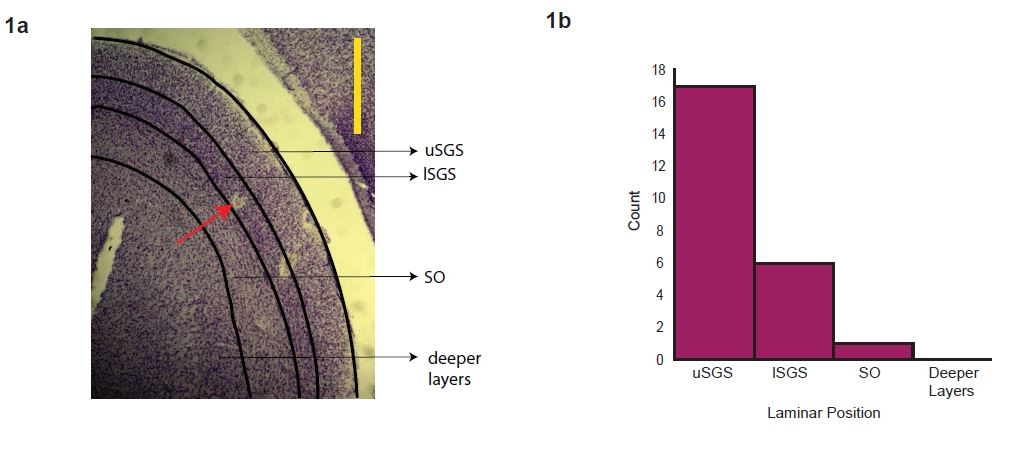
\includegraphics[width=\linewidth]{SCLaminarPosition.jpg}
		\caption{Histology. a) A section of tree shrew superior colliculus showing electrolytic lesions. Red arrow
			points to an electrolytic lesion. Scale bar (yellow vertical line) denotes 1000 μm. b) A summary of laminar
			position of recorded units in the superior colliculus. Abbreviations: uSGS- upper Stratum Griseum Superficiale;
			lSGS- lower Stratum Griseum Superficiale; SO- Stratum Opticum.}
		\label{fig:fig1}
	\end{figure}
	
	
	
	\subsubsection{Orientation Selectivity}
	
		The response of a representative neuron to moving bars of different orientations and the corresponding orientation tuning curves are presented in figure showed in figure 6.2. The response was the average of 10 trials and the small error bars suggest that the response was highly consistent (Error bars = $\pm$ sem). The CV of this neurons was 0.82. The median CV of all the neurons in our sample was 0.82 with a range of [0.29, 0.94]. Any neuron with CV greater than 0.9 was considered not selective to orientation. Two neurons had a CV greater than 0.9 and were excluded from further analysis. The orientation tuning curves of the most selective, least selective neuron with Cv less than 0.9 and the least selective neuron in the entire sample are presented in figure 6.3. The histogram of all the circular variances are presented in figure 6.4.
	
	\begin{figure}
		
		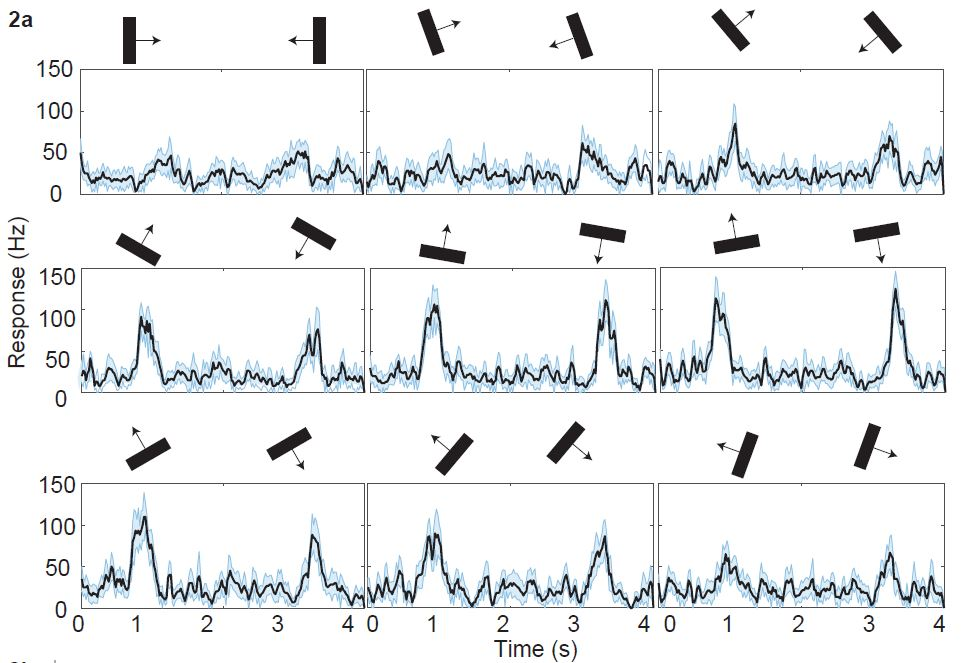
\includegraphics[width=\linewidth]{SCOriResp.jpg}
		\caption{Orientation response of an example cell.
			2a) Spike density functions (20 ms bins smoothed over
			3 bins) of the neuron’s response to oriented bar (direction
			of motion above each peak).}
		\label{fig:fig2}
	\end{figure}
	
	
	\begin{figure}
		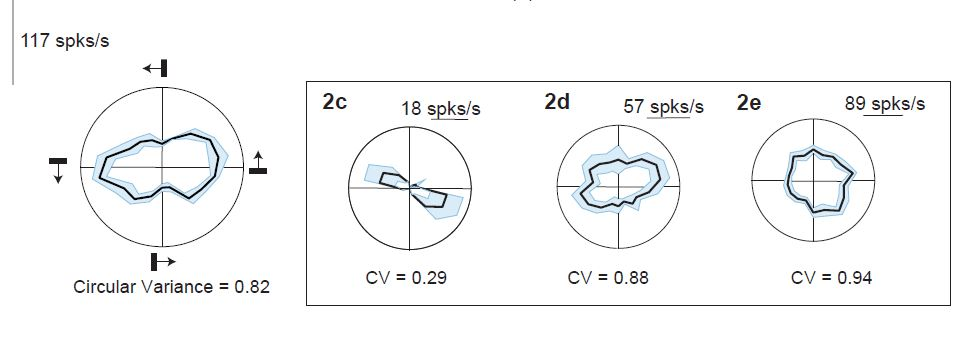
\includegraphics[width=\linewidth]{SCOriTuning.jpg}
		\caption{Polar plot showing
			the orientation tuning of the bar. Error bars denote
			Standard error. Orientation tuning curves of the
			sharpest (2c) and the least tuned (2d) neurons
			included in our analysis. (2e) was the least tuned
			neuron in our sample}
		\label{fig:fig3}			
	\end{figure}
	

	\begin{figure}
		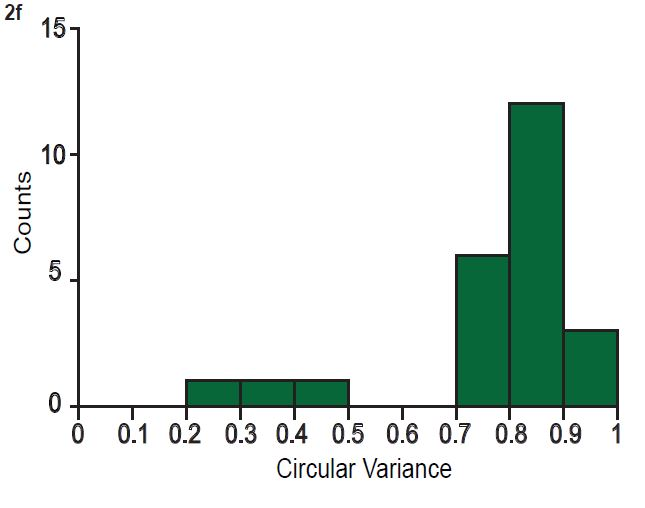
\includegraphics[width=\linewidth]{SCCircVar.jpg}
		\caption{This figure demonstrates the distribution of circular
			variances of all neurons.}
		\label{fig:fig4}			
	\end{figure}
	
	
	
	\subsubsection{Spatial Frequency Tuning}
	When the spatial frequency tuning response of the neuron at different orientations was observed, 13 of 16 neurons were orientation tuned at higher spatial frequencies. The spatial frequency response of an example neuron at the optimum and the orthogonal orientations is presented in figure 6.5a. The response is the F0 component of the FFT. The gray shaded area represents the spatial frequnecies where the neuron still responds to the optimum orientation but no longer responds to the orthogonal orientation (ie. the neuron is orientation tuned).  The upper limit of the gray shaded area (the dotted line to the right) is the cut off spatial frequency at the optimum orientation. The sf corresponding to the lower limit of the shaded gray area is the cut off spatial frquency. The difference in response between the optimum and non-optimum orientation cut off frequencies was calculated. These results for the group are presented in figure 6.6 a. On average, the response to the orthogonal orientation reached the minimum 0.5 cpd before the response to the optimum orientation; with the 95 percent CI= [0.4, 0.6].
	
	The OSI at each of the spatial frequencies for the example neuron is plotted in figure 6.5 b and the group results are presented in figure 6.6 b.
	The neuron exhibited the highest bias close to the cut off frequency at the orthogonal orientation.
	
	\begin{figure}
		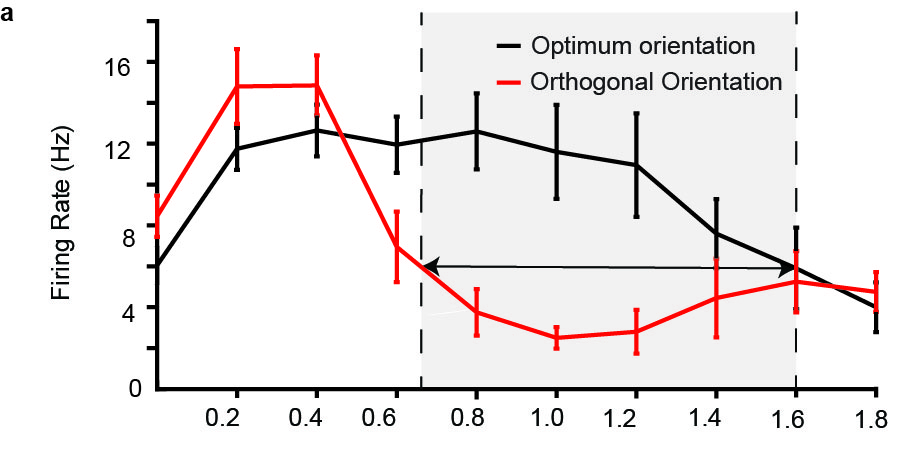
\includegraphics[width=\linewidth]{SCOptOrth.jpg}
		\caption{Example SF tuning curves for optimal and orthogonal orientations. The cut-off frequency at the
			optimal orientation is the SF at which the response at optimal orientation is no longer significantly different from the response at orthogonal
			orientation. The response at the cut-off frequency for optimum orientation is called the minimum response. For the orthogonal orientation, the
			cut-off frequency was the SF at which minimum response was first reached.}
		\label{fig:fig5}			
	\end{figure}
	
	\begin{figure}
		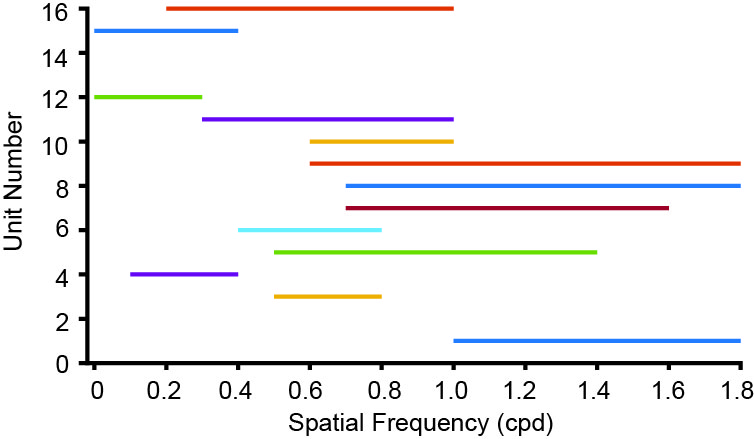
\includegraphics[width=\linewidth]{SCSFTuning.jpg}
		\caption{ The difference between the cut-off frequencies for the optimum
			and orthogonal orientations for 16 units is shown in Figure 3b.}
		\label{fig:fig6}			
	\end{figure}
	
	\begin{figure}
		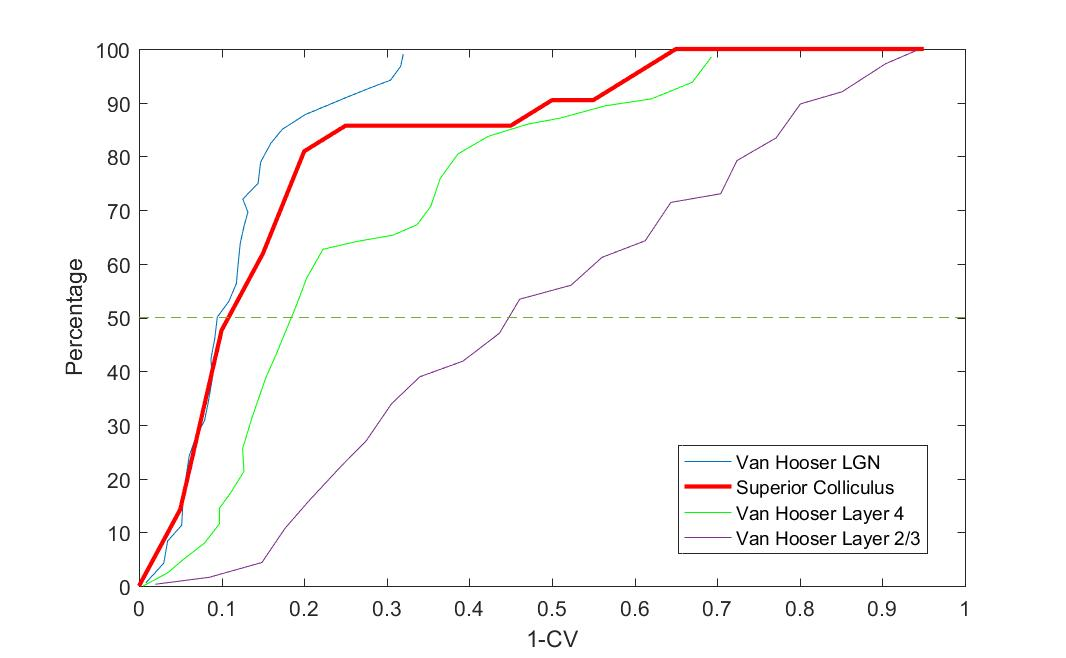
\includegraphics[width=\linewidth]{SCvgeniculostriate.jpg}
		\caption{ Comparison of the Superior Colliculus vs neurons in the geniculostriate system (data collected by Van Hooser et al., 2013)}
		\label{fig:fig7}			
	\end{figure}
	
	
	\section{Discussion}
	
		The histology confirmed that all the units that were recorded from the superficial layers of the superior colliculus. While the superior colliculus receives information from all the sensory modalities, the superficial layers receive direct input from the retina and feedback projections from the primary visual cortex. They also project to extrastriate visual areas. Lesion studies have shown that when the shrew SC is lesioned, form perception is affected. In Studies where the primary visual cortex of the tree shrew was ablated while keeping the SC and extra-striate visual areas intact showed that tree shrews could still consciously perceive form information further implicating the superficial layers of the shrew SC in playing an important role in perception. Given its position in this alternate visual pathway and its role in form perception, it is surprising that orientation tuning has not been reported in the Superior Colliculus. Where it has been reported, like in the case of the tree shrews, a very small proportion of neurons have said to be tuned to orientation. These neurons have also been reported in the superficial areas of the superior colliculus. 
		
		In their earlier paper, Albano et al., 1978 suggested that less that 10\% of the neurons had elongated receptive fields. However, in our study, 90\% of our neurons were orientation selective. It is important to make a distinction in these two results. While they may sound like it, these results are not entirely contradictory. In their study, Albano et al tested the elongation of the receptive fields. That is, using the neuronal responses, they plotted the receptive field boundaries of neurons and concluded that any neuron that had an aspect ration of 3:1 had elongated receptive field. In this study on the other hand, we used the response of the neurons to bars and gratings of different orientations. Studies have shown that only a slight receptive field elongation is required for a neuron to give orientation specific response. Albano et al may have simply not detected smaller effects which have been reported in the retina and LGN due to their conservative criterion for classifying a neuron as orientation selective.
		
		Another reason Albano et al., 1978 may not have detected the extent of orientation tuning in the shrew SC could be the stimulus used. As mentioned earlier, bars and gratings were used in this study. Albano et al also used these stimuli however, only one paper was published (1974) in the cat retina indicating that orientation tuning was detected at higher spatial frequencies (Hammond, 1974). However, in the eighties, a lot of papers were published revealing the spatial frequency dependence of orientation tuning. The lack of this knowledge may also be one of the reasons why the orientation selectivity in the superior colliculus was missed.
		
		One of the prominent paper published investigating the spatial frequency dependence of orientation tuning in the retinal ganglion cells of cats was Levick and Thibos (1982). They characterised the way orientation tuning varied with spatial frequency. In the following paragraph, I will evaluate our results in the context of the responses of retinal ganglion cells.
		
		One of the two key findings of Levick and Thibos was that RGCs were tuned to orientation at higher spatial frequencies. They also found that in some cases, at lower spatial frequencies, the neuron responded better at the orthogonal orientation compared to optimal orientation. They also reported that the degree of orientation selectivity (reported as orientation bias) was the maximum close to the threshold. In the tree shrew SC, all these findings hold true. A close examination of Fig: 6.5 shows that orientation tuning is observed at higher spatial frequencies. Figure 6.5 b also shows that the orientation bias was the maximum close to the threshold. Figure 6.6 also demonstrates this. Figure 6.5 is also only one example of a case where the neuron was biased for the orthogonal orientation at lower spatial frequencies. 
		
				
		
	
	\subsection{Anatomical Relevance}
	
	What did you find?
	Orientaiton bias in the superior colliculus at higher spatial frequencies.
	So what?
	well orientation bias is in the retina.
	Ok?
	And everyone thinks that orientation selectivity is generated in the cortex.
	So what does this show?
	It shows that orientation selectivity is present earlier in the visual system. 
	Is this the first time that's been shown?
	No. It's been shown in the LGN and in the retina.
	OK? So what's new?
	Reporting orientation bias in the superior colliculus means that orientation bias is probably inherited from the retina.
	So what?
	Being present earlier in the visual system means that the visual system doesn't have to reinvent the wheel over and over again.
	
	\subsection{Orientation selectivity in shrew superior colliculus}
	\subsection{Direction selectivity}
	\subsection{Similarities and differences with other species}
	